\section{Preselection yields}
\label{sec:yields}

Based on the event and trigger selections described in~Section \ref{sec:eventSelection}, 
we define a preselection as follows:
\begin{itemize}
\item Number of jets $\geq$ 2
\item Same flavor dileptons (opposite flavor yields will be shown since 
  they are used in data for \ttbar background estimation)
%\item All dilepton flavor combinations (SF as well as OF) %I think this is misleading
\item Dilepton mass within 10~GeV of the Z mass
%\item Dilepton mass within 15~GeV of the \Z mass
\end{itemize}
The resulting dilepton mass spectra for the $ee$ and $\mu\mu$ final states are shown in Figure~\ref{fig:dilmass}.
%Add statement about overflow
For this plot and all others in this note, the last bin contains the overflow.

\begin{figure}[hbt]
  \begin{center}
	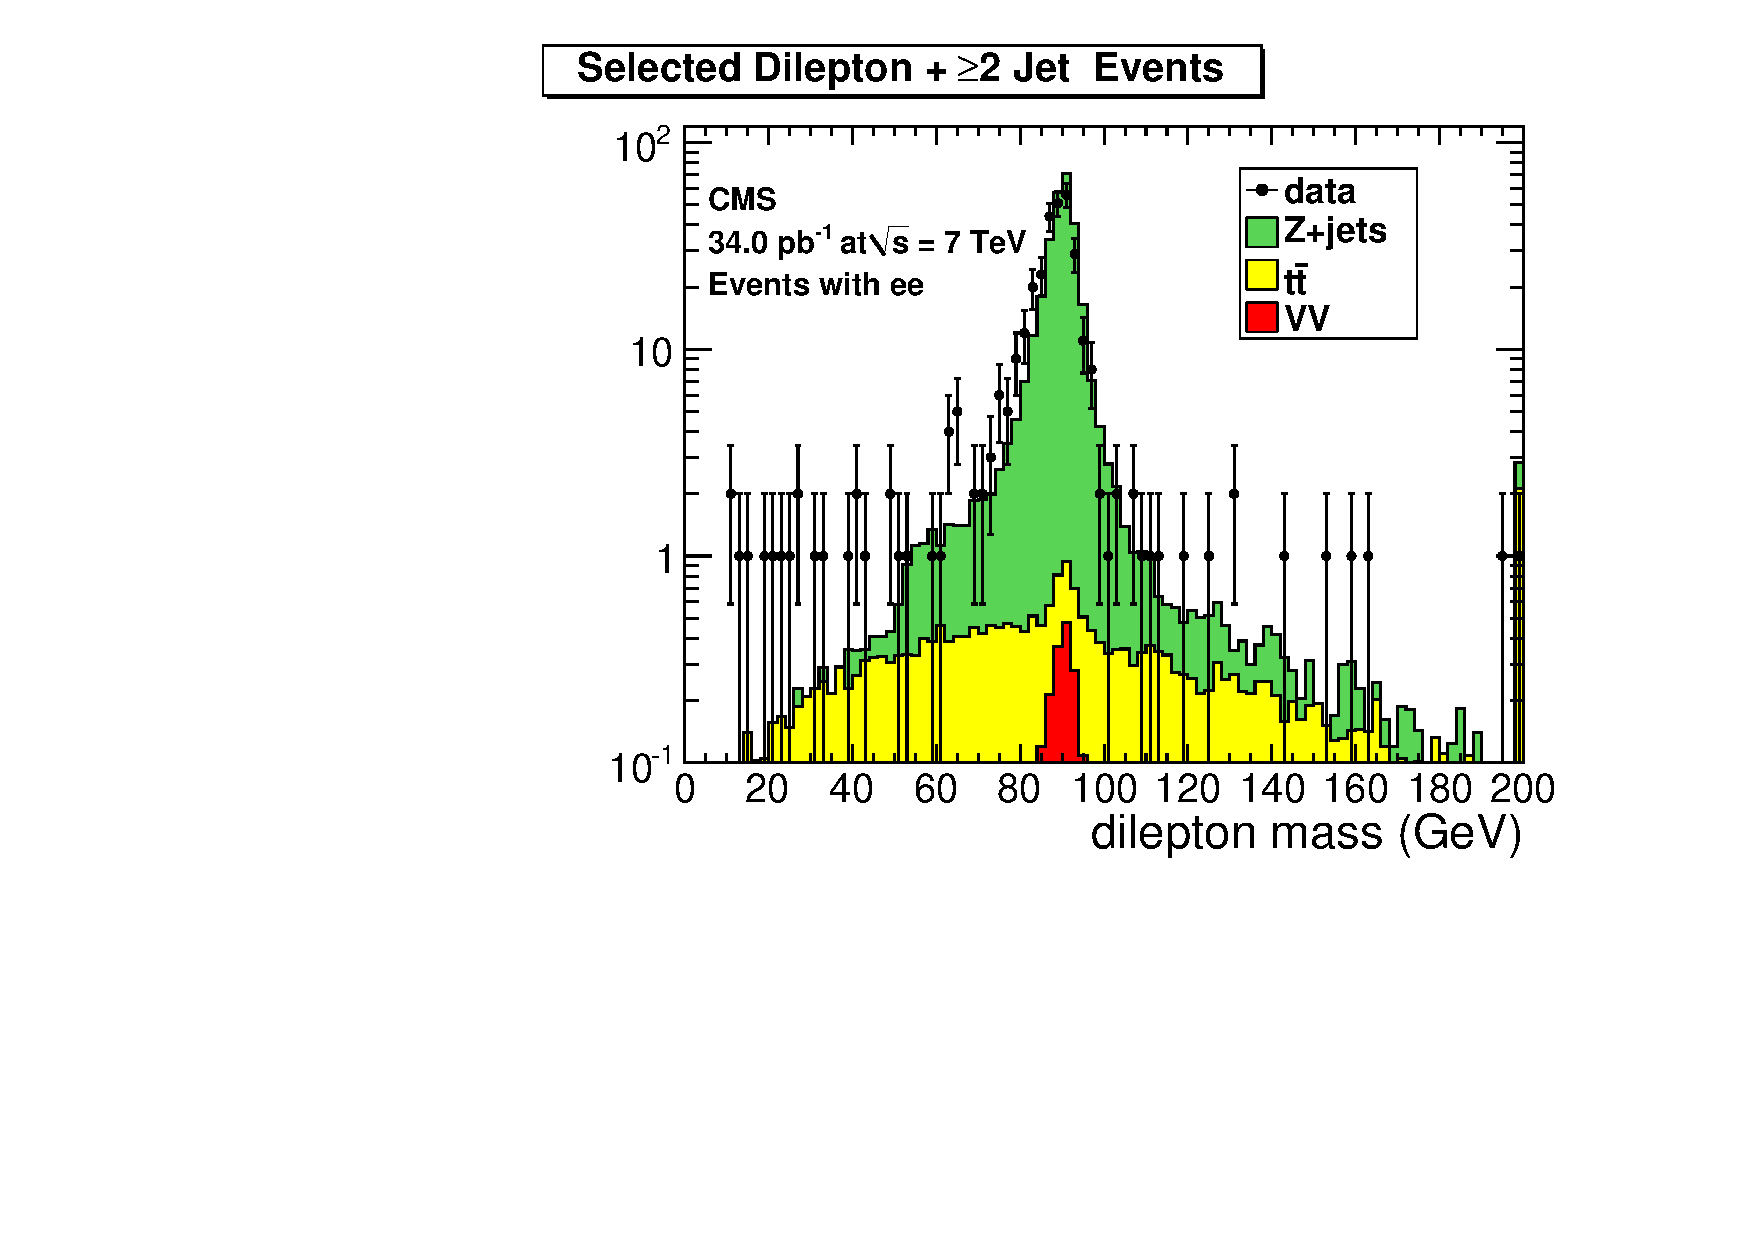
\includegraphics[width=0.48\linewidth]{plots/hdilmass_ee_allj.pdf}
	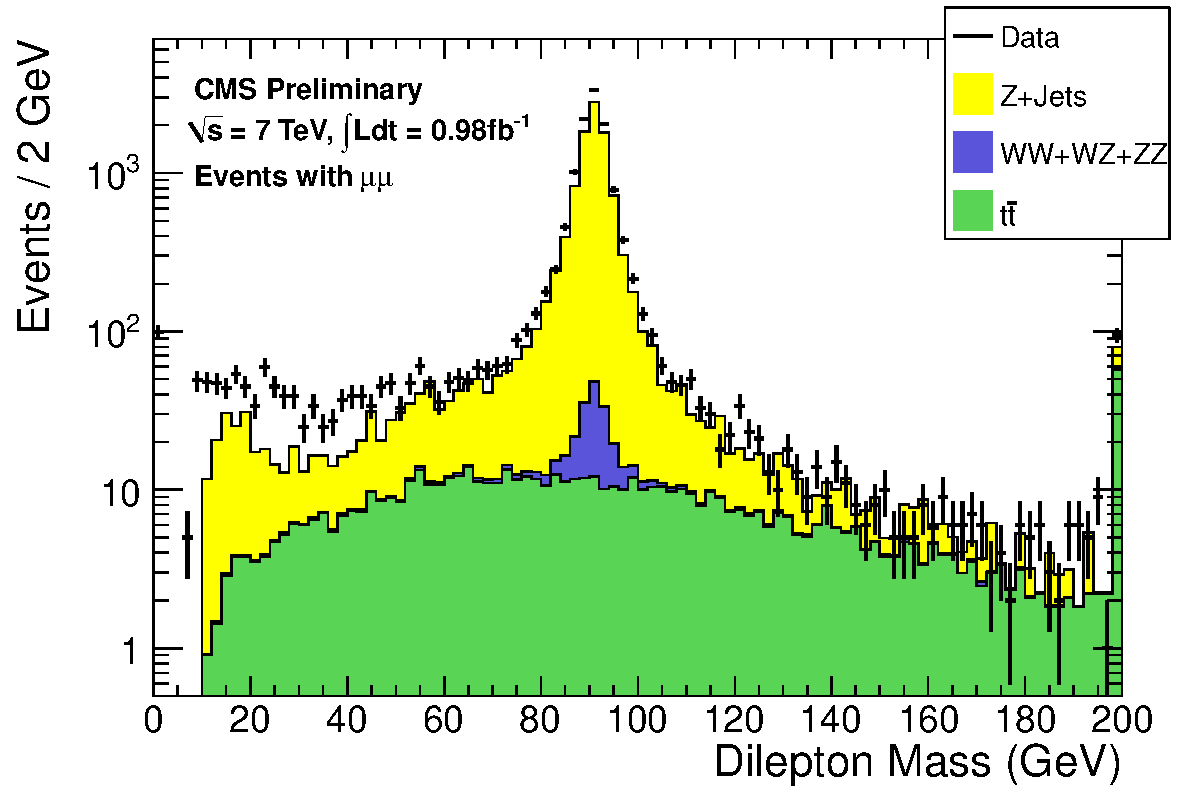
\includegraphics[width=0.48\linewidth]{plots/hdilmass_mm_allj.pdf}
	\caption{
	  \label{fig:dilmass}\protect 
	  Dilepton mass distribution for events passing the pre-selection for \lumi~
	  in the $ee$ (left) and $\mu\mu$ (right) final states. Backgrounds from 
	  single top and $W$+jets are omitted
	  since they are negligible.}
  \end{center}
\end{figure}


%\begin{figure}[htb]
%  \begin{center}
%    \resizebox{0.6\linewidth}{!}{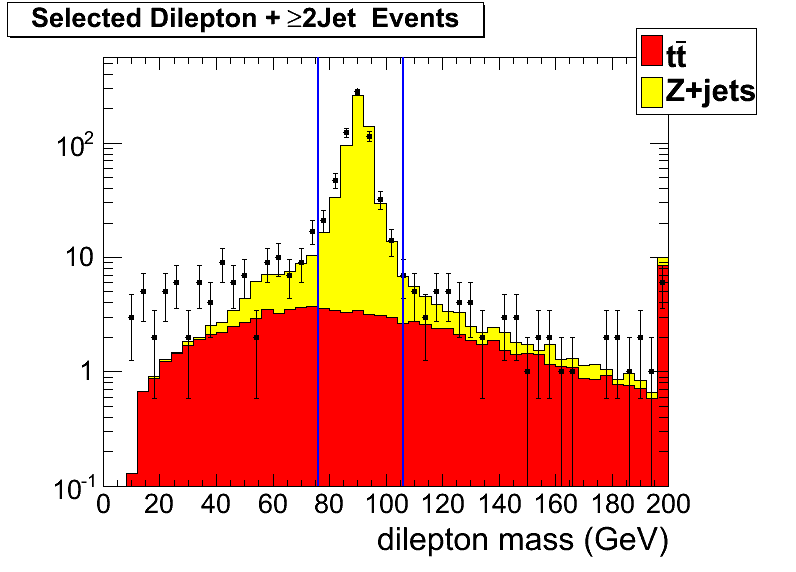
\includegraphics{plots/dilmass_34pb.png}}
%    \caption{ \label{fig:dilmass} Dilepton mass distribution for events passing the pre-selection for \lumi.}
%  \end{center}
%\end{figure}


The data yields and the MC predictions are given in Table~\ref{preselyieldtable}.

The MC yields are normalized to \lumi\ using the cross-sections
from Reference~\cite{ref:xsec} assuming 100\% trigger efficiency 
%{\bf(will have to fix this next pass)} 
.
As anticipated, the MC predicts that the preselection is dominated by Z+jets in the same-flavor 
case and by \ttbar in the opposite-flavor case.  
%The data yield is in reasonable agreement with the predictions for the $ee$, $\mu\mu$ and $e\mu$ channels.
We also show the %LO 
next-to-leading order (NLO) %don't have these yet, but should get
yields for the LM4 and LM8 processes, which are benchmark
SUSY processes in which $Z$ bosons are produced via cascade decays of SUSY particles. 

%, while an excess of 
%data events is observed in the $\mu\mu$ case. 
%We believe that this is due to a slightly harder njet distribution in data vs MC, combined with a slight 
%deficiency of electron yield with respect to MC. {\bf Reevaluate w new mc}

%I'm replacing below with above

%{\bf NOTE: This excess was not understood, and we investigated it a bit.
%In the 11/pb sample it is a difference between the Njet spectra between e/mu. It mostly went away in the 35/pb sample. We do see a difference in yield in the later data between e/mu, though - To be investigated. Maybe reReco will fix that. }

\begin{table}[htb]
\begin{center}
\caption{\label{preselyieldtable} Data and Monte Carlo yields for the preselection for \lumi. 
  The NLO yields for the SUSY benchmark processes LM4 and LM8 are also shown.}
\begin{tabular}{lccccc}
\hline
              Sample   &                $ee$   &            $\mu\mu$   &              $e\mu$   &                 tot  \\
\hline
       Z+Jets & 1840.566 $\pm$ 21.213  &  2088.019 $\pm$ 22.592  &   1.467 $\pm$  0.599  &  3930.052 $\pm$ 30.996 \\ 
   $t\bar{t}$ & 24.515 $\pm$  0.860  &  25.965 $\pm$  0.885  &  51.295 $\pm$  1.244  &  101.775 $\pm$  1.753 \\ 
        WJets &  0.852 $\pm$  0.603  &   0.000 $\pm$  0.000  &   0.426 $\pm$  0.426  &   1.278 $\pm$  0.738 \\ 
           WW &  0.217 $\pm$  0.043  &   0.442 $\pm$  0.061  &   0.593 $\pm$  0.070  &   1.252 $\pm$  0.102 \\ 
           WZ & 13.947 $\pm$  0.157  &  16.001 $\pm$  0.168  &   0.111 $\pm$  0.014  &  30.059 $\pm$  0.230 \\ 
           ZZ & 10.005 $\pm$  0.076  &  11.364 $\pm$  0.082  &   0.022 $\pm$  0.004  &  21.391 $\pm$  0.112 \\ 
   Single Top &  0.725 $\pm$  0.057  &   0.778 $\pm$  0.059  &   1.694 $\pm$  0.088  &   3.196 $\pm$  0.120 \\ 
\hline
     Total MC & 1890.827 $\pm$ 21.240  &  2142.569 $\pm$ 22.610  &  55.607 $\pm$  1.450  &  4089.003 $\pm$ 31.056 \\ 
\hline
         Data &   2051                 &    2277                 &      66               &    4394 \\ 
\hline
          LM4 &  2.842 $\pm$  0.086  &   2.986 $\pm$  0.087  &   0.434 $\pm$  0.036  &   6.262 $\pm$  0.127 \\ 
          LM8 &  1.286 $\pm$  0.037  &   1.443 $\pm$  0.039  &   0.430 $\pm$  0.023  &   3.159 $\pm$  0.059 \\ 

%LO
%          LM4 &  2.027 $\pm$  0.060  &   2.175 $\pm$  0.062  &   0.291 $\pm$  0.023  &   4.493 $\pm$  0.089 \\ 
%          LM8 &  0.889 $\pm$  0.025  &   1.004 $\pm$  0.026  &   0.273 $\pm$  0.014  &   2.167 $\pm$  0.038 \\ 

\hline
\end{tabular}
\end{center}
\end{table}



%2010
%%%official PVT json v3, 38X MC 
%               ZJets   &   260.79 $\pm$ 3.29   &   282.49 $\pm$ 3.42   &     0.12 $\pm$ 0.07   &   543.39 $\pm$ 4.75  \\
%               TTbar   &     3.93 $\pm$ 0.12   &     4.01 $\pm$ 0.12   &     8.36 $\pm$ 0.18   &    16.30 $\pm$ 0.25  \\
%               WJets   &     0.19 $\pm$ 0.13   &     0.00 $\pm$ 0.00   &     0.09 $\pm$ 0.09   &     0.28 $\pm$ 0.16  \\
%                  WW   &     0.03 $\pm$ 0.01   &     0.05 $\pm$ 0.01   &     0.08 $\pm$ 0.01   &     0.15 $\pm$ 0.01  \\
%                  WZ   &     0.17 $\pm$ 0.01   &     0.18 $\pm$ 0.01   &     0.01 $\pm$ 0.00   &     0.36 $\pm$ 0.01  \\
%                  ZZ   &     1.54 $\pm$ 0.01   &     1.71 $\pm$ 0.01   &     0.00 $\pm$ 0.00   &     3.26 $\pm$ 0.02  \\
%                  tW   &     0.12 $\pm$ 0.01   &     0.11 $\pm$ 0.01   &     0.27 $\pm$ 0.01   &     0.51 $\pm$ 0.02  \\
%\hline
%           tot SM MC   &   266.78 $\pm$ 3.30   &   288.56 $\pm$ 3.43   &     8.94 $\pm$ 0.22   &   564.26 $\pm$ 4.76  \\
%\hline
%                data   &                 249   &                 331   &                   7   &                 587  \\
%\hline
%                 LM4   &     0.48 $\pm$ 0.01   &     0.51 $\pm$ 0.01   &     0.08 $\pm$ 0.01   &     1.06 $\pm$ 0.02  \\
%                 LM8   &     0.22 $\pm$ 0.01   &     0.25 $\pm$ 0.01   &     0.08 $\pm$ 0.00   &     0.55 $\pm$ 0.01  \\
